\chapter{Descrição da Implementação}
Neste capítulo, serão dados detalhes de como os conceitos do capitulo anterior foram implementados na prática, da descrição geral do sistema e dos resultados obtidos.
Nota-se, que os conceitos utilizados descritos, não são dependentes da plataforma e ferramentas especificas utilizadas para a solução encontrada, assim, discussões acerca do uso das ferramentas específicas também serão abordadas, tais como seus pontos positivos e negativos.


\section{Arquitetura do sistema}
% \todo{Fazer diagrama do funcionamento}
O sistema proposto será constituído de diversas partes que integram tanto software, quando hardware e firmware, como visto no diagrama abaixo.

\section{Hardware}
Após resultados positivos, com a prova de conceito, optou-se por seguir na mesma linha de hardware, utilizando-se microcontroladores da familia nRF5 que possuem bluetooth integrado. Após pesquisas entre hardwares que usavam tal chip e a possibilidade de desenvolvimento de um hardware próprio, chegou-se à conclusão de que, com a finalidade de minimizar erros, a melhor opção seria a busca por hardwares capazes de realizar a tarefa de localização eficientemente. Isto é, dispositivos que possuem um preço acessível, uma alta eficiencia energética e escalabilidade.

Com esses requisitos, um dispositivo que se mostrou como uma boa opção foi o \textit{Dev SmartScanner} e o \textit{DEV SmartTag} da empresa DEV Tecnologia \cite{DEV_Site}, \textit{designhouse} brasileira com foco om IoT. Após uma parceria com a empresa, foi possível obter alguns desses dispositivos, com a finalidade de melhorias no sistema de localização e integração com a localização em armazéns, característica muito desejada, porém que ainda não havia sido feita com esse dispositivo.

O \textit{DEV SmartTag} consiste em um \textit{beacon} que possui um \textit{hardware} simples, composto por um microcontrolador com bluetooth integrado, uma bateria e um medidor de bateria. Esse dispositivo tem uma única funcionalidade: emitir sinal de bluetooth.
Esse sinal é capturado pelo \textit{Dev SmartScanner} e transmitido para internet por meio de uma rede sem fio, de forma que o processamento dos algorimos de localizaçao aconteça na nuvem. O \textit{Dev SmartScanner} é composto principalmente por um microcontrolador equipado com bluetooth, para ser capaz de receber sinal do beacon e por um módulo Wi-Fi com capacidade de comunição com a internet. Ele não é alimentado por bateria, mas sim por uma fonte, já que  parte-se do pressuposto que de que ele fique em localização fixa e os tags que se mexem.

\begin{figure}[H]
	\centering
	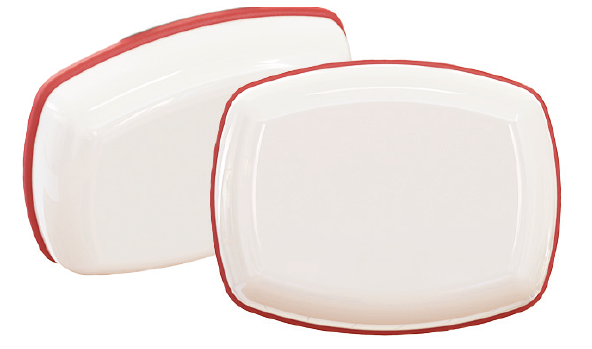
\includegraphics[scale = 1]{images/dev_tag.png}
	\caption{Aparência do \textit{DEV SmartTag}}
	\label{fig:dev_smart_tag}
\end{figure}

\begin{figure}[H]
	\centering
	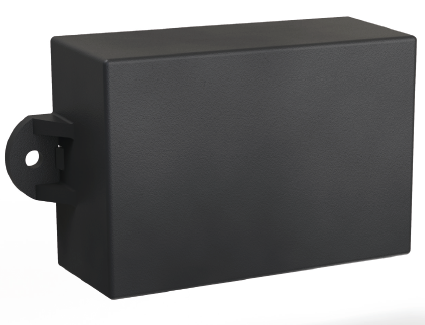
\includegraphics[scale = 1]{images/dev_scanner.png}
	\caption{Aparência do \textit{DEV SmartScanner}}
	\label{fig:dev_smart_scanner}
\end{figure}

Outras opções levantadas de \textit{hardware} que possibilitariam o uso específico para localização indoor de armazéns encontram-se na tabela abaixo:

\begin{table}[H]
    \centering
    \begin{tabular}{||c c c c c||}
    \hline
    Empresa & Modelo & Preço (USD) & Versão BLE & Link \\ [0.5ex]
    \hline\hline
    DEVTecnologia & DEV SmartTag & 35 & 4.1 & \cite{DEV_Site}\\
    \hline
    Kontakt & Tough Beacon & 25  & 4.2 & \cite{Kontakt_Site}\\
    \hline
    Beaconstac & Pocket & 23  & 4.0 & \cite{Beaconstac_Site}\\
    \hline
    Estimote & Proximity & 25 & 4.2 & \cite{Estimote_Site}\\
    \hline
    Quuppa & Q17 & -  & 5.1 & \cite{Quuppa_Site}\\ [0.5ex]
    \hline
    \end{tabular}
    \caption{Comparação hardwares comerciais}
    \label{tab: Tabela Comercial}
\end{table}


Apesar do preço um pouco mais elevado comercialmente e de não utilizar as especificações mais modernas de bluetooth (como a solução da Quuppa) a vantagem do hardware escolhido é que no trabalho foi possível ter acesso ao código fonte e fazer as modificações necessárias especificas na localização de ativos em um armazém. Além disso, foi o único hardware encontrado que foi desenvolvido no Brasil e que possui especificação Anatel, o que facilita a utilização e suporte em território brasileiro.

Além do hardware escolhido, cabe uma atenção especial ao Quuppa \cite{Quuppa_Site}. Essa empresa, é a pioneira no desenvolvimento de técnicas de localização indoor e atuou diretamente junto com o Bluetooth SIG no desenvolvimento de especificações atuais do bluetooth foco em localização indoor. Por ser uma empresa desse porte, suas soluções acabam saíndo por um preço alto, entretando uma boa precisão de localização é obtida.

\subsection{Especificações técnicas}
O DEV SmartScanner possui as seguintes especificações técnicas:


- Microcontrolador
% - Bateria
% - Tamanho
% - rendimento
% - alcance do sinal
% - array de antenas
% - features (ethernet)

\section{Back-end}
O sistema de localização deve se comunicar com o sistema do armazém de forma que os dados coletados possam ser usados com alguma finalidade. Dessa forma, é necessário uma forma de comunicação com algum sistema de gerenciamento de armazéns, que no caso é o sistema da samsung logistcs.

Para fazer essa integração o hardware é capaz de se conectar a internet e enviar pacotes de mensagens a algum servidor. Isso é feito com base em MQTT e o programa de back-end é feito em Go, para adquirir esses dados do MQTT.



\section{Funcionalidade}
\section{Resultados}
